%! Date = 18/07/2022

\documentclass[a4paper,11pt,draft=false]{scrartcl} % scrartcl scrreprt scrbook

\usepackage{ebgaramond} % gillius ebgaramond
\usepackage{amsmath}
\usepackage[ngerman]{babel}
\usepackage{relsize}
\usepackage{caption}
\usepackage{tabularx}
\usepackage[newfloat=true]{minted}
\usepackage{pdfpages}
\usepackage[utf8]{inputenc}
\usepackage[automake]{glossaries-extra}
\usepackage[onehalfspacing]{setspace}
\usepackage{graphicx}
\usepackage{biblatex}

%\bibliographystyle{plain} % We choose the "plain" reference style
% \usepackage{listings}
\bibliography{refs} % Entries are in the refs.bib file

%\newcommand{\heading}[1]{\multicolumn{1}{c}{#1}}
% \renewcommand{\lstlistingname}{Auflistung}
\setlength{\parindent}{0pt} % disable weird indentation after \begin...\end sections for now
\graphicspath{ {./images/} }

\makeglossaries

\newglossaryentry{Textpassage}
{
    name=Textpassage,
    description={Ein Stück Text aus einer Textdatei. Dabei
            wird sich meist auf eine in der Konfigurationsdatei spezifizierte
            Zieldatei des Programms bezogen.}
}

\newglossaryentry{Zielmuster}
{
    name=Zielmuster,
    description={Ein Element innerhalb der Konfigurationsdatei. Es bezeichnet ein
            Stück Text das einen speziellen \gls{Platzhalter}, den Text \mintinline{bash}{{{value}}},
            enhält. Es wird vom Programm dazu genutzt den genauen Ort der Ziel-\gls{Textpassage}
            innerhalb der Zieldatei zu identifizieren. Das Zielmuster sollte}
}

\newglossaryentry{Platzhalter}
{
    name=Platzhalter,
    description={Ein vordefinierter Text: das englische Wort \mintinline{bash}{value}
            umgeben von doppelten geschweiften Klammern:
            \mintinline{bash}{{{value}}} Das Format des Platzhalters ist an die
            die Template-Engine Template-Engine Jinja2 \cite{jinja2} angelehnt.
            Er ist Teil des \gls{Zielmuster}s das zusätzlich Text vor und nach
            der Ziel-\gls{Textpassage} enthält. Er markiert den Ort der Ziel-\gls{Textpassage}
            relativ zum \gls{Zielmuster} innerhalb der Zieldatei.}
}

\newglossaryentry{Property-Based-Testing}
{
    name=Property-Based-Testing,
    description={Property-Based-Testing bezeichnet eine spezielle Strategie Softwaretests
            zu formulieren. Statt einer Reihe explizit ausformulierter Tests wird eine Regel
            formuliert, welcher das zu testende Programm für automatisch generierte Eingabewerte
            genügen muss.}
}

\glsaddall

\author{Adrian Schurz}
\title{Terminal-Config-Manager\\
	Informatik für Anwendungsentwicklung\\
	CHECK24 Tech Hub und Services GmbH\\
	}

\begin{document}

\definecolor{codebg}{rgb}{0.95,0.95,0.95}

\maketitle
\pagenumbering{gobble}
\newpage

\section{Projektantrag}
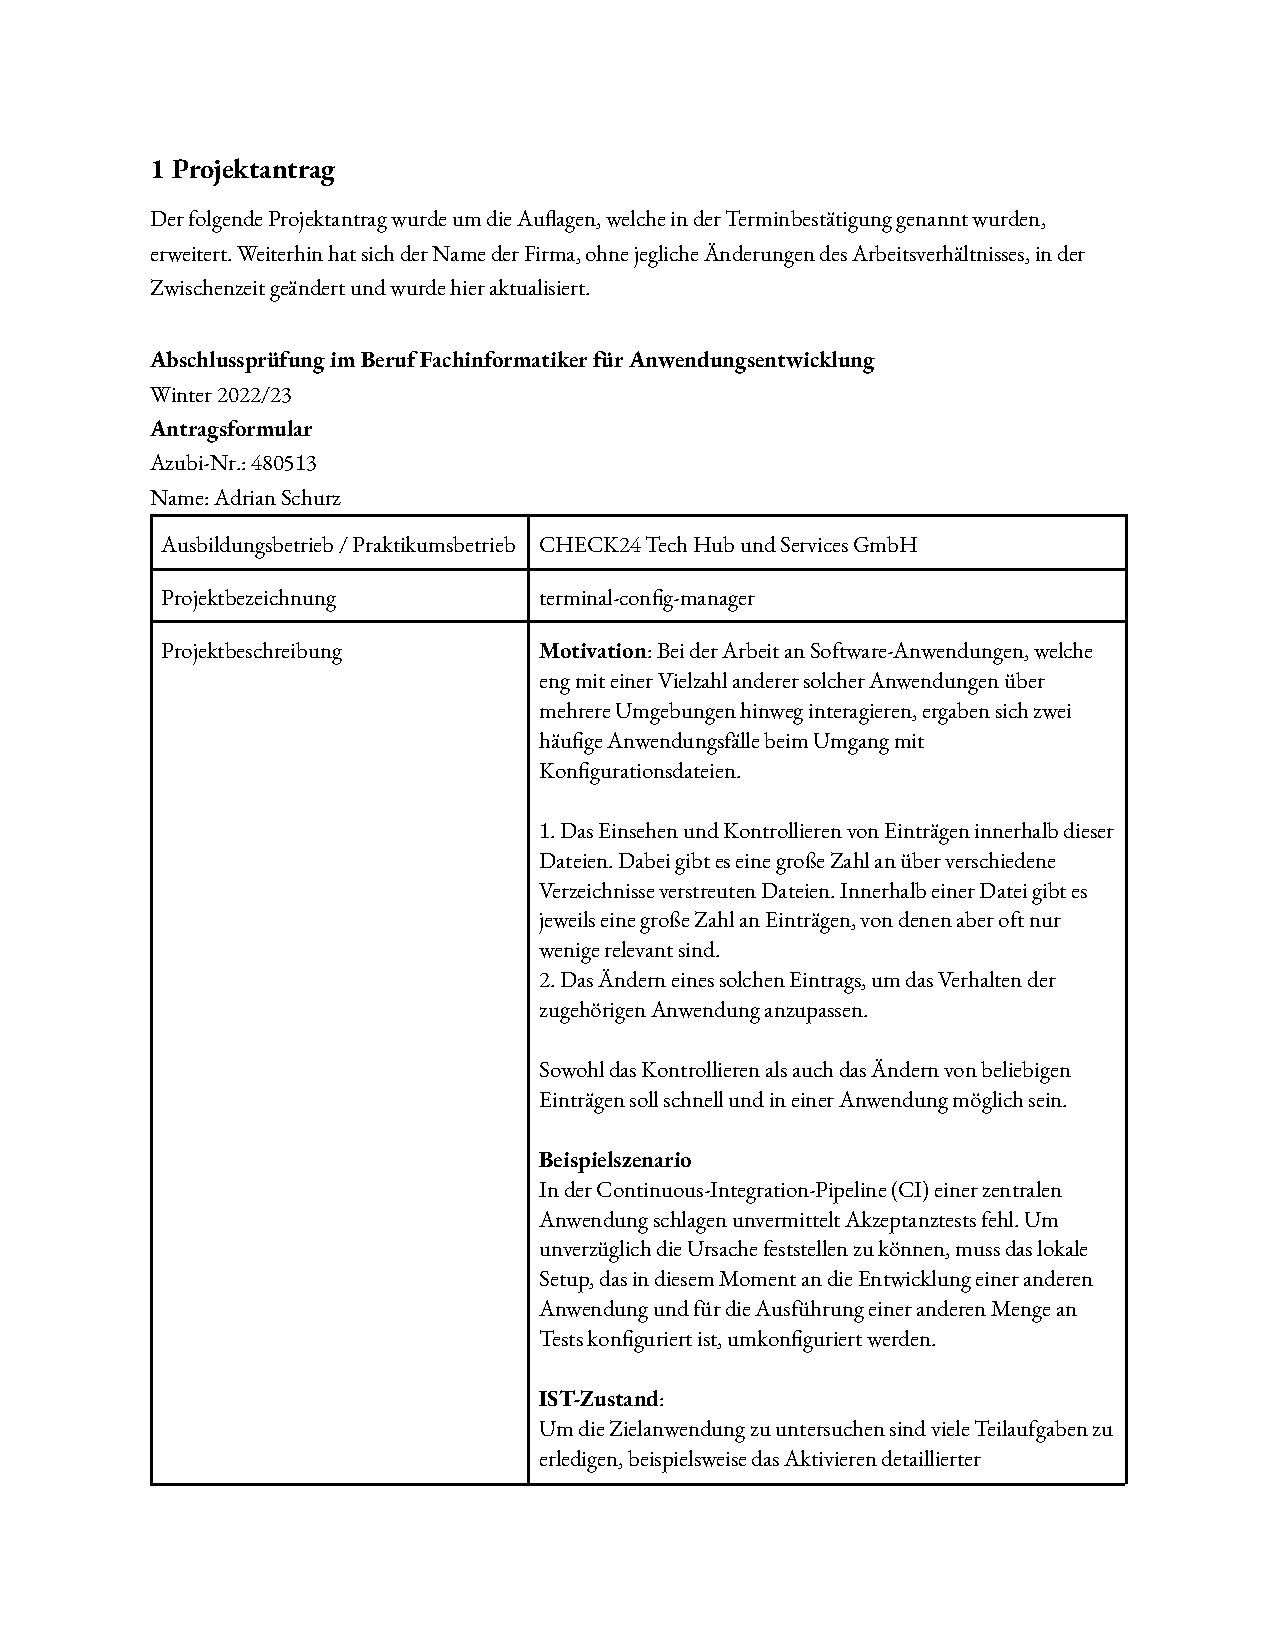
\includepdf[pages={-}]{../projektantrag/projektantrag_final.pdf}

\section{Nachweisblatt}
\paragraph{}

\newpage
\tableofcontents
\newpage

% Textteil
\pagenumbering{arabic}

\section{Problemstellung}

\section{Literaturverzeichnis}

\section{Anlagen}

\section{Kundendokumentation}

\subsection{Beschreibung}
Terminal-Config-Manager ist ein Linux-Programm mit welchem
\gls{Textpassage}n innerhalb meherer Dateien schnell zwischen einer Reihe
vorkonfigurierter \gls{Textpassage}n umgeschalten werden können.

Der Hauptanwendungsfall ist die effiziente  Manipulation von
Konfigurationsdateien von Softwareanwendungen, die häufig angepasst
werden müssen.

\subsection{Installation} \label{Installation}
Es wurden vorkonfigurierte Pakete für sowohl ArchLinux\cite{arch}-basierte als auch
Debian\cite{debian}-basierte Betriebssysteme bereitgestellt. Alternativ
kann das Programm auch manuell installiert werden.

\begin{center}
	\textbf{Arch-Linux \cite{arch}, via PKGBUILD Datei und pacman \cite{pacman}}
\end{center}

Im Projektverzeichnis unter

\begin{minted}[bgcolor=codebg]{bash}
	/distribution/arch/PKGBUILD
\end{minted}

befindet sich eine Spezifikationsdatei anhand derer das Softwarepaket
erstellt und anschließend installiert werden kann:

\begin{minted}[bgcolor=codebg]{bash}
	cd distribution/arch
	makepkg
	pacman -U terminal-config-manager-1.0.0-1-x86_64.pkg.tar.zst
\end{minted}

Die Deinstallation erfolgt mittels

\begin{minted}[bgcolor=codebg]{bash}
	pacman -R terminal-config-manager
\end{minted}

\begin{center}
	\textbf{Debian, via .deb Datei und dpkg\cite{dpkg}  bzw. apt\cite{apt}}
\end{center}

Im Projektverzeichnis unter

\begin{minted}[bgcolor=codebg]{bash}
	/distribution/debian/terminal-config-manager.deb
\end{minted}

befindet sich ein Softwarepaket, das mittels \mintinline{bash}{dpkg}
oder \mintinline{bash}{apt} direkt installiert werden kann.

\begin{minted}[bgcolor=codebg]{bash}
	cd distribution/debian
	dpkg --install ./terminal-config-manager.deb
	# apt install ./terminal-config-manager.deb
\end{minted}

Die Deinstallation erfolgt mittels

\begin{minted}[bgcolor=codebg]{bash}
	dpkg --remove terminal-config-manager
	# apt remove terminal-config-manager
\end{minted}

\begin{center}
	\textbf{Alternative, ohne Paketmanager}
\end{center}

Wenn das Programm nicht vom systemeigenen Paketmanager verwaltet werden
soll, dann kann es manuell kompiliert und in einem passenden
Verzeichnis abgelegt werden.

Voraussetzung hierfür ist, dass das Programm \mintinline{bash}{stack} auf dem
System installiert ist.

Im Projektverzeichnis wird mit

\begin{minted}[bgcolor=codebg]{bash}
	stack build --test --copy-bins
\end{minted}

das Programm kompiliert, die Testsuite ausgeführt und die ausführbare Datei im
Projektverzeichnis unter

\begin{minted}[bgcolor=codebg]{bash}
	bin/terminal-config-manager
\end{minted}

abgelegt. Anschließend kann das Programm in ein Verzeichnis kopiert werden, das in die
Systempfadliste eingetragen ist, beispielsweise

\begin{minted}[bgcolor=codebg]{bash}
	cp bin/terminal-config-manager ~/.local/bin
\end{minted}

Die Deinstallation erfolgt mittels

\begin{minted}[bgcolor=codebg]{bash}
	rm ~/.local/bin/terminal-config-manager
	rm <Konfigurationsdateipfad>
\end{minted}

\subsection{Konfiguration}
Die Zieldateien und -textpassagen müssen vor Ausführung des Programms
über eine Datei im YAML-Format konfiguriert werden.

\paragraph{Verzeichnis}
Das Programm erwartet, dass sich eine solche Datei in einem der folgenden
Verzeichnisse befindet. Die Reihenfolge entspricht der absteigenden Priorität
beim Vorhandensein mehrerer Konfigurationsdateien:

\begin{enumerate}
  \item ./config.yaml
  \item \$\{HOME\}/.config/terminal-config-manager/config.yaml \textbf{(empfohlen)}
  \item \$\{HOME\}/.terminal-config-manager.yaml
\end{enumerate}

Der Dateipfad 1 bezeichnet den Ort der ausführbaren Datei selbst und sollte nur
zu Debugging- oder Entwicklungszecken genutzt werden. Die Pfade 2 und 3 sind
gängige Ablageorte für nutzerspezifische Konfigurationsdateien unter Linux.

\newenvironment{code}{\captionsetup{type=listing}}{}
\SetupFloatingEnvironment{listing}{name=Abbildung}

\begin{figure}
  \caption{Beispielaufbau der Konfigurationsdatei}
  \label{fig:sample-config}
  \begin{minted}[bgcolor=codebg]{yaml}
    config_lines_to_manage:
      - title: Beispieltitel 1
        path: /home/alice/zieldatei.conf
        pattern: "'statspush_enabled' => {{value}},"
        targetValue: "true"
        possibleValues:
          - "true"
          - "false"

      - title: Beispieltitel 2
        path: /home/alice/verzeichnis/weitere-zieldatei.txt
        pattern: "SOFTWARE_ENV={{value}}"
        targetValue: production
        possibleValues:
          - testing
          - staging
          - production
          - local

      - ...
  \end{minted}
\end{figure}

\paragraph{Aufbau}
In Abb. \ref{fig:sample-config} ist der Aufbau der Konfigurationsdatei
illustriert. In \cite{latex2e}

\subsection{Benutzung} \label{Benutzung}
\paragraph{Start}
Das Programm wird nach erfolgreicher Installation mit dem Befehl

\begin{minted}[bgcolor=codebg]{bash}
    terminal-config-manager
\end{minted}

von der Kommandozeile aus gestartet. Für jeden Eintrag in der Konfigurationsdatei
zeigt das Programm eine Zeile an.

\begin{figure}
    \caption{Ansicht nach Programmstart}
    \label{post-start}
    \begin{center}
        \fbox{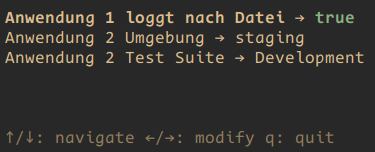
\includegraphics[scale=0.5]{post-start.png}}
    \end{center}
\end{figure}

\paragraph{Ansicht}
Abb. \ref{post-start} zeigt eine typische Ansicht direkt nach dem Start des
Programms. Die ersten drei Zeilen repräsentieren jeweils einen Eintrag in
der Konfigurationsdatei und somit eine Ziel-\gls{Textpassage} mit ihrem
aktuellen Wert. Jede dieser Zeilen besteht aus dem in der Konfigurationsdatei
vergebenen Titel des Eintrags, einem Pfeil und dem aktuellen Wert der Ziel-\gls{Textpassage}.
Die \textbf{aktuell ausgewählte Zeile} ist fett gedruckt während
\textcolor{teal}{der aktuelle Wert} der ausgewählten Zeile blau dargestellt wird.
Die genaue Darstellung ist dabei vom verwendeten Terminal-Emulator und dessen
Einstellungen bezüglich Schriftart und Farbwerten abhängig.

\paragraph{}
Die ausgegraute Zeile am unteren Rand beschreibt in Kurzform die verfügbaren
Kommandos und die davon ausgelösten Aktionen.

\paragraph{Aktionen}
Die Hauptfunktionen werden über die vier Pfeiltasten gesteuert. Die Pfeiltasten
hoch bzw. runter bewegen die Zeilenmarkierung nach oben bzw. unten. Die Pfeiltasten
links bzw. rechts schalten den zur markierten Zeile gehörigen Wert weiter zum
nächsten Wert aus der konfigurierten Liste der möglichen Werte
(siehe Kapitel \ref{Konfiguration} - Konfiguration). Beim Umschalten eines Werts
wird die zugehörige Zieldatei entsprechend modifiziert.

\paragraph{} Mit einem Tastendruck auf q kann das Programm jederzeit beendet werden
und zur Kommandozeile zurückgekehrt werden.

\subsection{Problembehandlung} \label{Problembehandlung}
\paragraph{Fehlende Konfigurationsdatei} Wenn beim Programmstart der Fehler
\begin{minted}[bgcolor=codebg]{bash}
    Error: No config file found at any of the search paths: ...
\end{minted}
auftritt, dann bedeutet das, dass bei der Suche nach Konfigurationsdateien an
keinem der angegebenen Pfade eine Datei gefunden wurde.
\paragraph{Lösung}
Es wird wie in Kapitel \ref{Konfiguration} (Konfiguration) beschrieben eine
Konfigurationsdatei an einem der validen Dateipfade angelegt. Im Dateisystempfad
unter

\begin{minted}[bgcolor=codebg]{bash}
    /usr/share/terminal-config-manager/config.yaml
\end{minted}

befindet sich eine Beispielkonfigurationsdatei, welche als Vorlage genutzt
werden kann:

\begin{minted}[bgcolor=codebg]{bash}
    mkdir ~/.config/terminal-config-manager
    cp  /usr/share/terminal-config-manager/config.yaml \
        ~/.config/terminal-config-manager
\end{minted}

\paragraph{Falsches Konfigurationsdateiformat} \label{missing-config} Wenn beim
Programmstart ein Fehler ähnlich

\begin{minted}[bgcolor=codebg]{text}
    An error occured while parsing the configuration file.
    The details are: ...
\end{minted}

auftritt, dann bedeutet das, dass die erste vom Programm gefundene Konfigurationsdatei
entweder nicht dem YAML-Format \cite{yaml} entspricht und/oder fehlende Elemente aufweist.

\paragraph{Lösung}
Die Fehlermeldung wird weitere Detailinformationen enthalten wie beispielsweise:

\begin{minted}[bgcolor=codebg]{text}
    The top level of the config file
    should be an object named 'config_lines_to_manage'
\end{minted}

anhand derer sich das Problem identifizieren lässt. Im Zweifelsfall muss dem
Kapitel \ref{Konfiguration} (Konfiguration) bzw. der Problembehandlung für
fehlende Konfigurationsdateien in Kapitel \ref{missing-config} folgend eine valide Konfigurationsdatei
per Hand angelegt werden.

\paragraph{Fehlende Dateizugriffsrechte} Wenn bei der Auswahl eines neuen Werts
der Fehler

\begin{minted}[bgcolor=codebg]{text}
    terminal-config-manager: <Zieldateipfad>: withFile:
    permission denied
\end{minted}

auftritt, dann bedeutet das, dass dem aktuellen Linux-Nutzer die nötigen
Zugriffsrechte fehlen, um die Zieldatei zu modifizieren.

\paragraph{Lösung}
Es muss sichergestellt werden, dass alle in der Konfigurationsdatei definierten
Zieldateien vom aktuellen Nutzer modifiziert werden können. Im häufigsten Fall
ist der aktuelle Nutzer nicht als \mintinline{bash}{owner} der Datei eingetragen:

\begin{itemize}
    \item Wenn dies angebracht ist, dann kann der Nutzer der Datei geändert werden:
          \begin{minted}[bgcolor=codebg]{text}
            chown <Nutzer> <Zieldateipfad>
        \end{minted}
    \item Wenn dies angebracht ist, dann können die Schreibrechte der Zieldatei
          angepasst werden:
          \begin{minted}[bgcolor=codebg]{text}
            chmod o+w <Zieldateipfad>
        \end{minted}
\end{itemize}

\textbf{Wenn keine der beiden oben genannten Optionen anwendbar ist, dann ist diese
    Zieldatei nicht für die Modifizierung durch das Programm geeignet}.

\printbibliography

\printglossaries

\end{document}